\documentclass[twoside]{book}

% Packages required by doxygen
\usepackage{fixltx2e}
\usepackage{calc}
\usepackage{doxygen}
\usepackage[export]{adjustbox} % also loads graphicx
\usepackage{graphicx}
\usepackage[utf8]{inputenc}
\usepackage{makeidx}
\usepackage{multicol}
\usepackage{multirow}
\PassOptionsToPackage{warn}{textcomp}
\usepackage{textcomp}
\usepackage[nointegrals]{wasysym}
\usepackage[table]{xcolor}

% Font selection
\usepackage[T1]{fontenc}
\usepackage[scaled=.90]{helvet}
\usepackage{courier}
\usepackage{amssymb}
\usepackage{sectsty}
\renewcommand{\familydefault}{\sfdefault}
\allsectionsfont{%
  \fontseries{bc}\selectfont%
  \color{darkgray}%
}
\renewcommand{\DoxyLabelFont}{%
  \fontseries{bc}\selectfont%
  \color{darkgray}%
}
\newcommand{\+}{\discretionary{\mbox{\scriptsize$\hookleftarrow$}}{}{}}

% Page & text layout
\usepackage{geometry}
\geometry{%
  a4paper,%
  top=2.5cm,%
  bottom=2.5cm,%
  left=2.5cm,%
  right=2.5cm%
}
\tolerance=750
\hfuzz=15pt
\hbadness=750
\setlength{\emergencystretch}{15pt}
\setlength{\parindent}{0cm}
\setlength{\parskip}{3ex plus 2ex minus 2ex}
\makeatletter
\renewcommand{\paragraph}{%
  \@startsection{paragraph}{4}{0ex}{-1.0ex}{1.0ex}{%
    \normalfont\normalsize\bfseries\SS@parafont%
  }%
}
\renewcommand{\subparagraph}{%
  \@startsection{subparagraph}{5}{0ex}{-1.0ex}{1.0ex}{%
    \normalfont\normalsize\bfseries\SS@subparafont%
  }%
}
\makeatother

% Headers & footers
\usepackage{fancyhdr}
\pagestyle{fancyplain}
\fancyhead[LE]{\fancyplain{}{\bfseries\thepage}}
\fancyhead[CE]{\fancyplain{}{}}
\fancyhead[RE]{\fancyplain{}{\bfseries\leftmark}}
\fancyhead[LO]{\fancyplain{}{\bfseries\rightmark}}
\fancyhead[CO]{\fancyplain{}{}}
\fancyhead[RO]{\fancyplain{}{\bfseries\thepage}}
\fancyfoot[LE]{\fancyplain{}{}}
\fancyfoot[CE]{\fancyplain{}{}}
\fancyfoot[RE]{\fancyplain{}{\bfseries\scriptsize Generated by Doxygen }}
\fancyfoot[LO]{\fancyplain{}{\bfseries\scriptsize Generated by Doxygen }}
\fancyfoot[CO]{\fancyplain{}{}}
\fancyfoot[RO]{\fancyplain{}{}}
\renewcommand{\footrulewidth}{0.4pt}
\renewcommand{\chaptermark}[1]{%
  \markboth{#1}{}%
}
\renewcommand{\sectionmark}[1]{%
  \markright{\thesection\ #1}%
}

% Indices & bibliography
\usepackage{natbib}
\usepackage[titles]{tocloft}
\setcounter{tocdepth}{3}
\setcounter{secnumdepth}{5}
\makeindex

% Hyperlinks (required, but should be loaded last)
\usepackage{ifpdf}
\ifpdf
  \usepackage[pdftex,pagebackref=true]{hyperref}
\else
  \usepackage[ps2pdf,pagebackref=true]{hyperref}
\fi
\hypersetup{%
  colorlinks=true,%
  linkcolor=blue,%
  citecolor=blue,%
  unicode%
}

% Custom commands
\newcommand{\clearemptydoublepage}{%
  \newpage{\pagestyle{empty}\cleardoublepage}%
}

\usepackage{caption}
\captionsetup{labelsep=space,justification=centering,font={bf},singlelinecheck=off,skip=4pt,position=top}

%===== C O N T E N T S =====

\begin{document}

% Titlepage & ToC
\hypersetup{pageanchor=false,
             bookmarksnumbered=true,
             pdfencoding=unicode
            }
\pagenumbering{alph}
\begin{titlepage}
\vspace*{7cm}
\begin{center}%
{\Large My Project }\\
\vspace*{1cm}
{\large Generated by Doxygen 1.8.13}\\
\end{center}
\end{titlepage}
\clearemptydoublepage
\pagenumbering{roman}
\tableofcontents
\clearemptydoublepage
\pagenumbering{arabic}
\hypersetup{pageanchor=true}

%--- Begin generated contents ---
\chapter{C\+S3560-\/final}
\label{md_README}
\Hypertarget{md_README}
Will be used for the final 
\chapter{File Index}
\section{File List}
Here is a list of all documented files with brief descriptions\+:\begin{DoxyCompactList}
\item\contentsline{section}{\hyperlink{counter_8cc}{counter.\+cc} \\*Counts the number of lines and the number of characters }{\pageref{counter_8cc}}{}
\end{DoxyCompactList}

\chapter{File Documentation}
\hypertarget{counter_8cc}{}\section{counter.\+cc File Reference}
\label{counter_8cc}\index{counter.\+cc@{counter.\+cc}}


counts the number of lines and the number of characters  


{\ttfamily \#include $<$iostream$>$}\newline
{\ttfamily \#include $<$fstream$>$}\newline
{\ttfamily \#include $<$string$>$}\newline
Include dependency graph for counter.\+cc\+:
\nopagebreak
\begin{figure}[H]
\begin{center}
\leavevmode
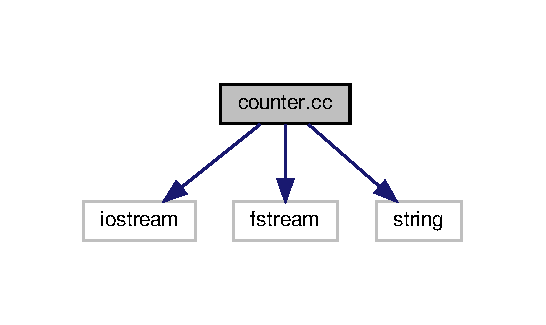
\includegraphics[width=262pt]{counter_8cc__incl}
\end{center}
\end{figure}
\subsection*{Functions}
\begin{DoxyCompactItemize}
\item 
int \hyperlink{counter_8cc_aef7d4c92788d40d516885f9759d709ac}{count\+Line} (string filename)
\begin{DoxyCompactList}\small\item\em counts the number of lines in the text files \end{DoxyCompactList}\item 
int \hyperlink{counter_8cc_afa6fb262a19b3fed61f78da61e705e65}{count\+Char} (string filename)
\begin{DoxyCompactList}\small\item\em counts the number of character, not including spaces, in the text files \end{DoxyCompactList}\item 
int \hyperlink{counter_8cc_a0ddf1224851353fc92bfbff6f499fa97}{main} (int argc, char $\ast$argv\mbox{[}$\,$\mbox{]})
\begin{DoxyCompactList}\small\item\em gets the file and calls the functions count\+Lines() and \hyperlink{counter_8cc_afa6fb262a19b3fed61f78da61e705e65}{count\+Char()} \end{DoxyCompactList}\end{DoxyCompactItemize}


\subsection{Detailed Description}
counts the number of lines and the number of characters 



\subsection{Function Documentation}
\mbox{\Hypertarget{counter_8cc_afa6fb262a19b3fed61f78da61e705e65}\label{counter_8cc_afa6fb262a19b3fed61f78da61e705e65}} 
\index{counter.\+cc@{counter.\+cc}!count\+Char@{count\+Char}}
\index{count\+Char@{count\+Char}!counter.\+cc@{counter.\+cc}}
\subsubsection{\texorpdfstring{count\+Char()}{countChar()}}
{\footnotesize\ttfamily int count\+Char (\begin{DoxyParamCaption}\item[{string}]{filename }\end{DoxyParamCaption})}



counts the number of character, not including spaces, in the text files 

\begin{DoxyReturn}{Returns}
int count -\/ the number of characters in the text file 
\end{DoxyReturn}
\mbox{\Hypertarget{counter_8cc_aef7d4c92788d40d516885f9759d709ac}\label{counter_8cc_aef7d4c92788d40d516885f9759d709ac}} 
\index{counter.\+cc@{counter.\+cc}!count\+Line@{count\+Line}}
\index{count\+Line@{count\+Line}!counter.\+cc@{counter.\+cc}}
\subsubsection{\texorpdfstring{count\+Line()}{countLine()}}
{\footnotesize\ttfamily int count\+Line (\begin{DoxyParamCaption}\item[{string}]{filename }\end{DoxyParamCaption})}



counts the number of lines in the text files 

\begin{DoxyReturn}{Returns}
int count -\/ the number of lines in the text file 
\end{DoxyReturn}
\mbox{\Hypertarget{counter_8cc_a0ddf1224851353fc92bfbff6f499fa97}\label{counter_8cc_a0ddf1224851353fc92bfbff6f499fa97}} 
\index{counter.\+cc@{counter.\+cc}!main@{main}}
\index{main@{main}!counter.\+cc@{counter.\+cc}}
\subsubsection{\texorpdfstring{main()}{main()}}
{\footnotesize\ttfamily int main (\begin{DoxyParamCaption}\item[{int}]{argc,  }\item[{char $\ast$}]{argv\mbox{[}$\,$\mbox{]} }\end{DoxyParamCaption})}



gets the file and calls the functions count\+Lines() and \hyperlink{counter_8cc_afa6fb262a19b3fed61f78da61e705e65}{count\+Char()} 

\begin{DoxyReturn}{Returns}
int -\/ 0 indicates a successful program run 
\end{DoxyReturn}

%--- End generated contents ---

% Index
\backmatter
\newpage
\phantomsection
\clearemptydoublepage
\addcontentsline{toc}{chapter}{Index}
\printindex

\end{document}
